% Literature Review
\glsresetall

This chapter delves deeper into the current \gls{sota} and the 
foundational work that has contributed to its development. 
It is divided into two main parts, the first a primer on relevant
background material and the second a review of related work.

The background is further divided into sections covering the foundational 
elements of reinforcement learning, the evolution to multi-agent systems
as the logical extension of single-agent \gls{rl}, 
the evolution to multi-agent systems from a game-theoretic perspective.
%
The related works is further divided into sections covering
the algorithms of interest, simulation environments,
and application papers.

% Surveys
% Algorithms
% Environments
% Applications

% #TODO:
% We need to do a related work section first.
% Cover the works that Directly inform ours
% Following the Related work, enter primer?

%\section{Related Work}


% ---------------------------------------------------------------------------- %
\section{Reinforcement Learning Foundations}%

    \subsection*{Markov Decision Processes}%

\Glspl{mdp} form the foundation of reinforcement learning by providing 
a formal framework for modeling decision-making in environments with 
stochastic dynamics~\cite{puterman2005}. An MDP is defined by a tuple 
(\gls{S}, \gls{A}, \gls{P}, \gls{R}, \gls{discount}), where:
\begin{itemize}
    \item \gls{S} is a finite set of states.
    \item \gls{A} is a finite set of actions.
    \item \(\gls{P}: S\times A\times S\rightarrow [0,1]\) is the state 
        transition probability function, where \(P(s^\prime|s, a)\) 
        represents the probability of transitioning to state \(s^\prime\in S\)
        given the current state \(s\in S\) and action \(a\in A\).
        This captures the stochastic nature of the environment.
    \item \(\gls{R}: S \times A \rightarrow \gls{reals}\) is the reward 
        function and written as \(R(s, a)\) defines the immediate reward 
        received after taking action \(a\in A\) in state \(s\in S\). 
        This reward guides the agent's learning process.
    \item \(\gls{discount} \in [0, 1]\) is the discount factor, which 
        determines the level of importance given to estimated future rewards. 
        Specifically, \(\gls{discount}=1\) implies that a reward estimate is 
        given equal value regardless of how many steps in the future it may 
        be while \(\gls{discount}=0\) implies that only the value of a 
        reward in the next step is considered.
\end{itemize}

\begin{figure}
    \centering
    \input{mdp_cycle}
    \caption{Fully reduced \glsentryshort{mdp} 
        representation of \glsentryshort{rl}.}
    \label{fig:mdp_cycle}
\end{figure}

    \subsection*{Objectives in MDPs}%

The objective in an \gls{mdp} is to find a policy 
\(\gls{pi}: \gls{S} \rightarrow \gls{A}\) that maximizes a return value. 
In the context of an episode it may be referred to as expected cumulative 
reward or \gls{etdr}, and in the context of a single time-step, 
the return \gls{G_t} at time \(t\) is defined as the sum of discounted rewards:
\begin{equation}
    \gls{G_t} = \sum_{k=0}^{\infty} \gls{discount}^k \gls{R}_{t+k+1}
    \label{eq:sum_discounted_rewards}
\end{equation}
where \(\gls{R}_{t+k+1}\) is the reward received following time step \(t+k\).
At the simplest level, reward is translated into a policy using either a 
value function; which may be a state-value or an action-value function 
(\cref{eq:state-value_function,eq:action-value_function} respectively).
A state-value function \gls{v_pi(s)} represents the expected return starting 
from state \(s\) and following policy \gls{pi}. It is generally defined as:
\begin{equation}
    \gls{v_pi(s)} 
    = \mathbb{E}_\pi [\gls{G_t}| \gls{S}_t = s] = \mathbb{E}_\pi \left[
        \sum_{k=0}^{\infty} \gls{discount}^k \gls{R}_{t+k+1} 
        \middle| \gls{S}_t = s \right]
    \label{eq:state-value_function}
\end{equation}
The action-value function \gls{q_pi(a|s)} represents the expected return 
starting from state \(s\), taking action \(a\), 
and thereafter following policy \gls{pi}:
\begin{equation}
    \gls{q_pi(a|s)} 
    = \mathbb{E}_\pi [\gls{G_t}| \gls{S}_t = s, \gls{A}_t = a] 
    = \mathbb{E}_\pi \left[ 
        \sum_{k=0}^{\infty} \gls{discount}^k \gls{R}_{t+k+1}
        \middle| \gls{S}_t=s, \gls{A}_t=a \right]
    \label{eq:action-value_function}
\end{equation}

    \subsection*{Bellman Equations and Optimal Policies}%

The Bellman equations provide recursive definitions for the value functions. 
\Cref{eq:bellman_state-value,eq:bellman_action-value} are the Bellman equations
of the state-value and action-value functions for a given policy \gls{pi} 
respectively.
\begin{equation}
    \gls{v_pi(s)} 
    = \sum_{a \in \gls{A}} \gls{pi}(a|s) 
      \sum_{s^\prime \in \gls{S}} \gls{P}(s^\prime|s, a) \left[
        \gls{R}(s, a) + \gls{discount} v_\pi(s^\prime)\right]
    \label{eq:bellman_state-value}
\end{equation} \begin{equation}
    \gls{q_pi(a|s)} 
    = \sum_{s^\prime \in \gls{S}} \gls{P}(s^\prime|s, a) \left[
        \gls{R}(s, a) + \gls{discount} \sum_{a^\prime \in \gls{A}} 
        \gls{pi}(a^\prime|s^\prime) q_\pi(s^\prime, a^\prime)\right]
    \label{eq:bellman_action-value} 
    \vspace*{1em}
\end{equation}
The goal is to find (or approximate) the optimal policy \gls{pi} that maximizes
the value functions for all states. The optimal Bellman equations are those that
satisfy \cref*{eq:bellman_optimal_state-value,eq:bellman_optimal_action-value}:
\begin{equation}
    \gls{v_*(s)} = \max_a \sum_{s^\prime \in \gls{S}} \gls{P}(s^\prime|s, a)
    [\gls{R}(s, a) + \gls{discount} v_*(s^\prime)]
    \label{eq:bellman_optimal_state-value}
\end{equation} \begin{equation}
    \gls{q_*(a|s)} = \sum_{s^\prime \in \gls{S}} \gls{P}(s^\prime|s, a) 
    [\gls{R}(s, a) + \gls{discount} \max_{a^\prime} q_*(s^\prime, a^\prime)]
    \label{eq:bellman_optimal_action-value}
\end{equation}

    \subsection*{Solution Methods}%

There are numerous methods for solving \glspl{mdp}, including exact methods 
like value iteration and policy iteration, as well as approximate methods 
such as \gls{rl} techniques. Exact methods iteratively compute the value 
functions and improve the policy until convergence to the optimal solution. 
However, for large state and action spaces, 
these methods become computationally infeasible.

In contrast, \gls{rl} methods, which develop policies through interaction
with the environment, offer a scalable approach for solving problems that
can be modelled as \glspl{mdp}. 
\Gls{rl} methods do not require a model of the environment's dynamics and can
handle large, complex problems where exact methods are intractable.
Before examining \gls{rl} approaches to multi-agent systems, we will cover 
several important concepts from the perspective of a single agent system.

% ---------------------------------------------------------------------------- %
\section{Single-Agent Reinforcement Learning}%

Single-agent \gls{rl} extends the foundational principles of \glspl{mdp} 
by enabling an agent to learn optimal policies through direct interaction with 
the environment. In single-agent \gls{rl}, the agent learns by trial and error, 
using feedback in the form of rewards to adjust its actions and maximize 
cumulative rewards over time.
Single-agent \gls{rl} employs various algorithms to learn the optimal policy by 
approximating the value functions. These algorithms can be broadly categorized 
into dynamic programming, Monte Carlo methods, and \gls{td} learning~%
\cite{sutton2018}.

    \subsection*{Dynamic Programming}%

Dynamic programming methods, such as value iteration and policy iteration, 
require a complete model of the environment's dynamics~\cite{sutton2018}.
They iteratively update value functions and policies until convergence. 
\textbf{Value Iteration} updates the value function based on the Bellman 
optimality equation until it converges to the optimal value function \(v_*\).
\textbf{Policy Iteration} alternates between policy evaluation 
(computing the value function for a fixed policy) and policy improvement 
(improving the policy based on the current value function) until convergence.

    \subsection*{Monte Carlo Methods}%

Monte Carlo methods learn directly from an agent's experience in an episode, 
estimating value functions by averaging the returns observed in actual episodes.
These methods are model-free and do not require knowledge of the environment's 
dynamics. They are generally divided into two categories; 
\textbf{First-Visit Monte Carlo}, averaging the returns of the first visit to 
each state, or \textbf{Every-Visit Monte Carlo}, averaging the returns of every
visit to each state in a given episode.
%
\begin{wrapfigure}[7]{R}{0.4\textwidth}
    \vspace*{-4em}
    \centering
    \resizebox{0.3\textwidth}{!}{%
        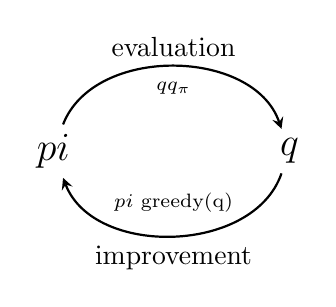
\begin{tikzpicture}[>=stealth, node distance=1.5cm, on grid, auto,
    arrow/.style = {thick,-stealth}]

    % States
    \node [] (center) {};
    \node [] (policy) [left=of center ] {\Large \(\gls{pi}\)};
    \node [] (values) [right=of center] {\Large \(\Gls{q}\)};

    % Transitions
    \draw [arrow] (policy) edge[bend left=70] node(E) {evaluation} (values);
    \draw [arrow] (values) edge[bend left=70] node(I) {improvement} (policy);
    \node [] () [below=15pt of E] {\scriptsize\(\Gls{q}\rightsquigarrow q_\pi\)};
    \node [] () [above=20pt of I] {\scriptsize\(\gls{pi}\rightsquigarrow\) 
        greedy(\Gls{q})};
\end{tikzpicture}
    }
    \captionsetup{margin=1.2em}
    \caption{Generalized Policy Iteration.}
    \label{fig:gpi_cycle}
\end{wrapfigure}
%
In either method, the policy and action values are updated iteratively.
Sutton and Barto~\cite{sutton2018} provide a graphic intuition for this 
iterative cycle, which we have replicated in~\cref{fig:gpi_cycle}.

A key distinction between Monte Carlo in this context and methods described 
later is that Monte Carlo methods execute an entire episode. In the following 
section, this principle will be applied to smaller segments of experience. 
Additionally, we will reference \gls{mcts}, 
a heuristic that simulates the results of future actions. Despite its name, 
\gls{mcts} is distinct from the Monte Carlo methods discussed here.

    \subsection*{Temporal-Difference (TD) Learning}%

\Gls{td} learning methods, such as Q-learning and SARSA 
(State-Action-Reward-State-Action), combine ideas from 
dynamic programming and Monte Carlo methods. They update value estimates 
based on observed transitions without waiting for the end of an episode.
Both methods use an \gls{step-size} parameter to determine the size of 
the update based on \cref{eq:action-value_function}.
%
\textbf{SARSA} is an on-policy \gls{td} control algorithm that updates the 
\gls{Q}-value using the \gls{Q}-value of the actual next state-action pair:
%
\begin{equation}
    \gls{Q}(s, a) \leftarrow \gls{Q}(s, a) + \gls{step-size} \left[ 
        \gls{R} + \gls{discount} \gls{Q}(s^\prime, a^\prime) - \gls{Q}(s, a) 
    \right]
    \label{eq:sarsa_action-value}
\end{equation}
%
\textbf{Q-Learning}~\cite{watkins1992} is an off-policy \gls{td} control 
algorithm that updates the \gls{Q}-value using the maximum \gls{Q}-value of 
from all actions available to the next state:
%
\begin{equation}
    \gls{Q}(s, a) \leftarrow \gls{Q}(s, a) + \gls{step-size} \left[ 
        \gls{R} + \gls{discount} \max_{a^\prime} 
        \gls{Q}(s^\prime, a^\prime) - \gls{Q}(s, a)
    \right]
    \label{eq:q-learning_action-value}
\end{equation}
%
Consequently, Q-learning has a tendency to converge faster than SARSA,
which may or may not be a desirable feature, depending on the needs
of the use-case.

    \subsection*{Exploration vs. Exploitation}

A fundamental challenge in \gls{rl}, as it is in all of machine learning, 
is balancing exploration (trying new actions to discover their effects) 
and exploitation (choosing actions known to yield high rewards). 
Common strategies for addressing this balance include \(\epsilon\)-greedy 
policies and Boltzmann exploration.
\(\epsilon\)-greedy increases the exploration of an algorithm by selecting
a random action \(\epsilon\) percent of the time.
%
Boltzmann exploration, commonly using a softmax function~\cite{pan2021}, 
normalizes estimated action-values to reduce bias during action selection. 
A temperature parameter \(\tau\) may be included to control the exploration 
rate over time, similar to a simulated annealing heuristic. 
%\Cref{eq:softmax_action-value} shows an example of this.
For example,
%
\begin{equation}
    P(A=a|S=s) =
    \frac{\exp\left\{\gls{Q}(a|s)/\tau\right\}}{
        \sum_{a^\prime\in A}\exp\left\{\gls{Q}(a^\prime|s)/\tau\right\}}
    \label{eq:softmax_action-value}
\end{equation}
However, Cesa-Bianchi et al.~\cite{cesa-bianchi2017} argue that this manner 
of implementation fails to minimize regret compared to \(\epsilon\)-greedy 
and attribute it to the difficulty in tuning a \(\tau\) decay schedule~
\cite{kaelbling1996,vermorel2005}.

% --- #TODO: Need a section on Neural Networks?

% ---------------------------------------------------------------------------- %
\section{Evolution to Multi-Agent Systems}%

The evolution from single-agent \gls{rl} to multi-agent systems introduces new 
complexities and opportunities, reflecting more realistic scenarios where 
multiple agents interact within a shared environment. \Gls{marl} extends the 
principles of single-agent RL to settings where agents must learn to 
cooperate, compete, or coexist, each influencing the other's learning process.
Key developments in centralized and decentralized training, communication and 
coordination, scalability, and stability have significantly expanded the 
applicability of \gls{marl} across various domains. 

    \subsection*{Cooperative Multi-Agent Systems}%

In cooperative multi-agent systems, agents work together to achieve a 
common goal. This requires coordination and communication to ensure that 
their actions complement each other. Cooperative MARL is often applied 
in tasks where the joint effort of multiple agents can lead to better 
performance than individual efforts~\cite{littman1994}.

The primary challenge in cooperative \gls{marl} is to develop 
strategies that maximize the collective reward~\cite{albrecht2024}. 
This involves a spectrum of approaches to the level of interaction 
between agents. Here we focus on interactions at the algorithmic level, 
rather than within the environment. On one end, 
a set of agents may be trained and deployed in a fully decentralized
manner~\cite{li2023d} and on the other,
we have integration such that the agents are simply copies of each other,
updating a shared policy~\cite{zheng2017}.

Rather than emphasizing either extreme, the majority of research in \gls{marl} 
has focused on leveraging interactions to produce more effective results. 
The most popular approaches fall under the label \gls{ctde}~%
\cite{foerster2017,rashid2018,fotouhi2019,lowe2020,pan2021,%
papoudakis2021,li2023d,zhou2023}, 
%
\begin{wrapfigure}[9]{R}{0.4\textwidth}
    \vspace*{-2.5em}
    \centering
    \documentclass{standalone}
\usepackage[dvipsnames]{xcolor}
\usepackage{tikz}
\usetikzlibrary{positioning, shapes, arrows,}

\begin{document}
\colorlet{DarkGreen}{Black!25!Green}
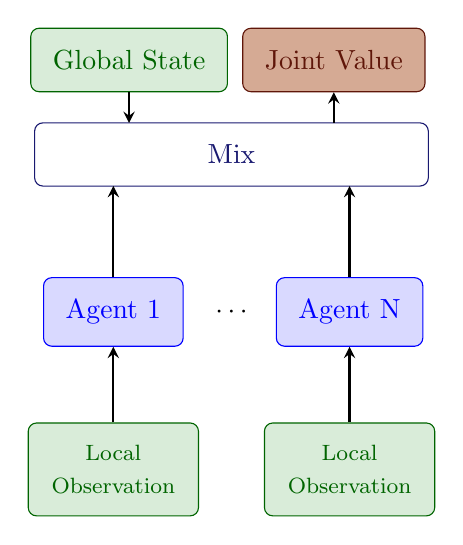
\begin{tikzpicture}[>=stealth, node distance=2cm, on grid, auto,
    entry/.style = {draw, rectangle, inner sep=8pt, rounded corners=3pt,
                    minimum width=1.5cm},
    greenEntry/.style = {draw, rectangle, inner sep=8pt, rounded corners=3pt,
                minimum width=1.5cm, align=center, DarkGreen, fill=Green!15},
    blueEntry/.style = {draw, rectangle, inner sep=8pt, rounded corners=3pt,
                    minimum width=1.5cm, Blue, fill=Blue!15},
    arrow/.style = {thick,-stealth}]

    % Entries
    \node [] (center) {\(\cdots\)};
    \node [blueEntry] (agent_1) [left =1.5cm of center] {Agent 1\ };
    \node [blueEntry] (agent_n) [right=1.5cm of center] {Agent N};
    \node [entry, MidnightBlue] (mix) [above=of center, minimum width=5cm] {Mix};
    \node [greenEntry] (state) [above left=1.2cm and 1.3cm of mix] 
        {Global State};
    \node [entry, Sepia, fill=Sepia!25] (value) [above right=1.2cm and 1.3cm of mix] {Joint Value};
    \node [greenEntry, text width=1.6cm] (obs_1) [below=of agent_1] 
        {\footnotesize Local Observation};
    \node [greenEntry, text width=1.6cm] (obs_n) [below=of agent_n] 
        {\footnotesize Local Observation};

    % Relations
    \draw [arrow] (obs_1) -- (agent_1);
    \draw [arrow] (obs_n) -- (agent_n);
    \draw [arrow] (agent_1) -- +(0,1.6);
    \draw [arrow] (agent_n) -- +(0,1.6);
    \draw [arrow] (state) -- +(0,-0.8);
    \draw [arrow] (value)+(0,-0.8) -- (value) ;
\end{tikzpicture}


\end{document}
    \caption{Basic \gls{ctde}.}
    \label{fig:basic_ctde}
\end{wrapfigure}
%
a broad term encompassing any algorithm with an arbitrary centralizing 
mechanism. We assert that the term's breadth and ubiquity have made it 
a defining trait of mainstream \gls{marl}.

Within the \gls{ctde} paradigm, we wish to draw particular attention to 
actor-critic training, derived from an almost identical single-agent 
training method. It is an intuitive implementation of \gls{ctde}, 
where the critic performs the role of mixing for the agents.

The majority of the algorithms we will examine in our experiments 
will either be actor-critic~\cite{foerster2017,lowe2020,li2023c} 
or will aim to reduce the bias that occurs with a singular, 
shared critic~\cite{rashid2018,ackermann2019,li2023d,zhou2023}.

\begin{wrapfigure}[9]{R}{0.4\textwidth}
    \vspace*{-1em}
    \centering
    \includegraphics[width=0.4\textwidth]{ctde_actor-critic.png}
    % #TODO:
    %\resizebox{0.3\textwidth}{!}{%
    %    % \documentclass{article}
% \usepackage{amsmath}
% \usepackage{tikz}
%     \usetikzlibrary{automata, positioning, calc, shapes.geometric, shapes.misc, fit}

% \begin{document}
% \providecommand{\gls}[1]{\ensuremath{#1}}
% \providecommand{\Gls}[1]{\ensuremath{\uppercase{#1}}}

\colorlet{SteelBlue}{blue!40!black!90}        % \definecolor{SteelBlue}{RGB}{70,130,180}
\colorlet{FireBrick}{red!60!black}            % \definecolor{FireBrick}{RGB}{178,34,34}
\colorlet{IndianRed}{red!40!brown}            % \definecolor{IndianRed}{RGB}{205,92,92}
\colorlet{OliveDrab}{green!80!brown!40!black} % \definecolor{OliveDrab}{RGB}{107,142,35}

\pgfdeclarelayer{agents}
\pgfdeclarelayer{execution}
\pgfdeclarelayer{training}
\pgfsetlayers{training, execution, agents, main}

\begin{tikzpicture}[>=stealth, node distance=3em, on grid, auto,
    arrow/.style = {very thick,-stealth}, ]

    % Placement references
    \node (C2) {\textcolor{SteelBlue}{\(\boldsymbol{\cdots}\)}};
    \node (C1) [above =1.3 of C2] {\textcolor{FireBrick}{\(\boldsymbol{\cdots}\)}};
    \node (C3) [below =1.5 of C2] {\textcolor{OliveDrab}{\(\boldsymbol{\cdots}\)}};

    %%% Agents %%%
    % A1
    \node[state, draw=SteelBlue!70,very thick,fill=SteelBlue!20] (A1) 
        [left =1.25 of C2] {\textcolor{SteelBlue}{\(\gls{a}_1\)}};
    % O1
    \node[state, draw=SteelBlue!70,very thick,fill=SteelBlue!20] (O1) 
        [left =of A1] {\textcolor{SteelBlue}{\(\gls{o}_1\)}};
    % Capsule 1
    \begin{pgfonlayer}{agents}
        \node[rounded rectangle, fill=IndianRed!40, fit=(A1)(O1), inner xsep=-2pt, 
            inner ysep=4pt] (Cap1) {};
    \end{pgfonlayer}
    % P1
    \path let \p1=(O1), \p2=(A1) in
        node[rectangle, draw=IndianRed!90,very thick,fill=IndianRed!40, inner sep=8pt, 
            minimum width={\x2-\x1+1.5em}] (P1) [above =1.3 of Cap1] 
            {\textcolor{FireBrick}{\(\gls{pi}_1\)}};
    % Q1
    \node[rectangle, draw=OliveDrab!90,very thick,fill=OliveDrab!40, inner sep=6pt] 
        (Q1) [below =1.5 of Cap1] {\textcolor{OliveDrab}{\(\Gls{q}_1\)}};

    % On
    \node[state, draw=SteelBlue!70,very thick,fill=SteelBlue!20] (On) 
        [right =1.25 of C2] {\textcolor{SteelBlue}{\(\gls{o}_n\)}};
    % An
    \node[state, draw=SteelBlue!70,very thick,fill=SteelBlue!20] (An) 
        [right =of On] {\textcolor{SteelBlue}{\(\gls{a}_n\)}};
    % Capsule n
    \begin{pgfonlayer}{agents}
        \node[rounded rectangle, fill=IndianRed!40, fit=(An)(On), inner xsep=-2pt, 
            inner ysep=4pt] (Capn) {};
    \end{pgfonlayer}
    % Pn
    \path let \p1=(On), \p2=(An) in
        node[rectangle, draw=IndianRed!90,very thick,fill=IndianRed!40, inner sep=8pt, 
            minimum width={\x2-\x1+1.5em}] (Pn) [above =1.3 of Capn] 
            {\textcolor{FireBrick}{\(\gls{pi}_n\)}};
    % Qn
    \node[rectangle, draw=OliveDrab!90,very thick,fill=OliveDrab!40, inner sep=6pt] 
        (Qn) [below =1.5 of Capn] {\textcolor{OliveDrab}{\(\Gls{q}_n\)}};
    

    %%% Interactions %%%
    % Q1 to P1
    \draw [arrow, draw=OliveDrab!60, rounded corners=0.75em] 
        (Q1.west) -- +(-1.1,0) coordinate(Q1P1) |- (P1.west);
    % Q1 to P1
    \draw [arrow, draw=OliveDrab!60, rounded corners=0.75em] 
        (Qn.east) -- +(1.1,0) coordinate(QnPn) |- (Pn.east);
    % Capsule 1 to Q1
    \draw [arrow, draw=OliveDrab!60] (Cap1.south) -- (Q1.north);
    % Capsule n to Qn
    \draw [arrow, draw=OliveDrab!60] (Capn.south) -- (Qn.north);
    % Capsule 1 to Qn
    \draw [arrow, draw=OliveDrab!60] 
        ([shift=({0.4,0.1})]Cap1.south east) -- ([shift=({-0.05,0.03})]Qn.north);
    % Capsule n to Q1
    \draw [arrow, draw=OliveDrab!60] 
        ([shift=({-0.4,0.1})]Capn.south west) -- ([shift=({0.05,0.03})]Q1.north);
    % O1 to P1
    \draw [arrow, draw=IndianRed!80] (O1.north) -- ($(O1.north |- P1.south)$);
    % P1 to A1
    \draw [arrow, draw=IndianRed!80] ($(A1.north |- P1.south)$) -- (A1.north);
    % On to Pn
    \draw [arrow, draw=IndianRed!80] (On.north) -- ($(On.north |- Pn.south)$);
    % Pn to An
    \draw [arrow, draw=IndianRed!80] ($(An.north |- Pn.south)$) -- (An.north);

    %%% Lower Layers %%%
    % Execution Layer
    \begin{pgfonlayer}{execution}
        \node[rectangle, rounded corners=1em, draw=FireBrick!75, dashed, very thick, 
            fill=IndianRed!20, fit=(P1)(Cap1)(Capn), inner sep=4pt, 
            inner ysep=4pt] (exec_box) {};
        \node[anchor=south] at (exec_box.north) (exec_label) 
            {\textcolor{FireBrick}{\textbf{Execution}}};
    \end{pgfonlayer}
    % Training Layer
    \begin{pgfonlayer}{training}
        \node[rectangle, rounded corners=1em, draw=OliveDrab!55, dashed, very thick, 
            fill=OliveDrab!5, fit=(exec_label)(Q1P1)(QnPn)(Qn), inner xsep=6pt, 
            inner ysep=4pt] (train_box) {};
        \node[anchor=south] at (train_box.north) (train_label) 
            {\textcolor{OliveDrab!75!green}{\textbf{Training}}};
    \end{pgfonlayer}

\end{tikzpicture}


% \end{document}
    %}
    %\captionsetup{margin=1.2em}
    \caption{Actor-Critic \gls{ctde}.}
    \label{fig:ctde_actor-critic}
\end{wrapfigure}

Rashid et al.~\cite*{rashid2018} and Li et al.~\cite*{li2023d}
proposed algorithms that decrease the amount of centralization 
of the critic functions, a change that will motivate later research
into \gls{harl} algorithms.

    %\subsection*{Competitive Multi-Agent Systems}
    % To fix a subsection to wrap figure collision.
    \paragraph*{\emph{Competitive Multi-Agent Systems}} \hfil 

In competitive multi-agent systems, agents have conflicting goals. 
The success of one agent typically comes at the expense of another,
and thus are often modeled as zero-sum games, where the gain of 
one agent is exactly balanced by the loss of another~\cite{leonardos2021}.

Thus competitive \gls{marl} typically involves strategies where agents 
must predict and counteract the actions of their opponents. 
Techniques from game theory, such as Nash equilibrium, are often employed 
to find stable strategies in these adversarial environments~\cite{busoniu2008}.

    \subsection*{Communication and Coordination}

Effective communication and coordination mechanisms are crucial 
for cooperative \gls{marl}. Agents need to share information and 
synchronize their actions to achieve common goals. 
Research in this area focuses on developing protocols and algorithms that 
enable efficient and robust communication among agents~%
\cite{sukhbaatar2016,fotouhi2019,hoang2023}.

    \subsection*{Scalability and Efficiency}

Scalability is a significant challenge in MARL due to the exponential 
growth of the state and action spaces with the number of agents~%
\cite{cao2012,busoniu2008}. 
Recent research efforts aim to develop algorithms that can efficiently 
scale to large numbers of agents and complex environments without 
compromising performance~\cite{smit2023,sun2023}.

    \subsection*{Stability and Convergence}

Ensuring the stability and convergence of learning algorithms in 
multi-agent settings is critical~\cite{papoudakis2021}. 
Unlike single-agent \gls{rl}, where convergence is well-understood, 
the dynamics of multiple learning agents can lead to instability 
and non-convergence. Research in this area seeks to establish 
theoretical guarantees and practical methods for stable learning.


% ---------------------------------------------------------------------------- %
\section{Evolution of MARL through the Lens of Games}%

Building upon these foundational advancements, the exploration of \gls{marl} 
through gameplay has provided a rich and challenging testbed for further 
innovation. Notably, the strategic complexity and real-time decision-making 
required in games have driven remarkable progress in \gls{marl} algorithms, 
as exemplified by pioneering projects such as 
DeepMind's AlphaGo\cite{silver2016}, AlphaGo Zero\cite{silver2017},
AlphaZero\cite{silver2017a} and AlphaStar\cite{vinyals2019}. 
These projects not only showcase the potential of \gls{marl} to 
achieve superhuman performance but also highlight the broader implications 
and applications of these advancements beyond the realm of gaming.

    \subsection*{AlphaGo: The First* Milestone}

AlphaGo, developed by DeepMind and presented in~\cite{silver2016}, 
marked perhaps the largest milestone in \gls{ai} since Deep Blue~%
\cite{campbell2002} with its victory over a world champion Go player.
Where Deep Blue was an expert system that leveraged an Alpha-Beta pruning 
algorithm and \glspl{asic} designed to execute the algorithm in parallel,
the state-space of Go was so much larger that this approach would not 
likely ever be tractable. AlphaGo achieved this success using 
\glspl{dnn} to approximating a value function and a policy.

An initial approximate policy was trained on 29.4 million states 
from 160,000 games using supervised gradient descent to predict 
the next move of a game given the current state.
An initial value function was approximated by sampling moves made 
during a game and assigning value according to the outcome of the game.
%
With initial approximate functions as a starting point,
a policy-gradient method in conjunction with \gls{mcts}
would provide the the framework for further improvement through \gls{rl}.

    \subsection*{AlphaGo Zero: A Leap Forward}

AlphaGo's success demonstrated the power of combining deep learning with 
traditional search techniques. However, the research team acknowledged potential
problems associated with the original approach's reliance on prepared data. 
In~\cite{silver2017}, Silver et al. express a concern regarding possible 
expense, unreliability, or unavailability of relevant data for pre-training.
They developed a new approach to address these concerns and titled it 
AlphaGo Zero. Here we focus on two key factors that made this possible.

First, the employment of the \gls{dnn} was simplified by combining the 
value function and policy into a single network that would take a state 
input and return a vector of move probabilities and a state value, 
this substantially reduced the cost of updating the network(s) during training.
%
Second, an increased reliance on training using self-play
eliminated the need for a collection of pre-played games.
Further, this reduced the influence that pre-established strategies 
used by human players would have on the training of the agent.

    \subsection*{AlphaStar: Expanding to Real-Time Strategy Games}

AlphaStar extended the principles of MARL to the domain of \gls{rts} 
games by achieving grandmaster-level performance in StarCraft II, 
a game known for its strategic depth, real-time decision-making, 
and partial observability. Vinyals et al.~\cite{vinyals2019} accomplished 
this using a large, modular neural network and a novel training curriculum.

The neural network interfaced with the game environment, which provided an 
observation space significantly larger than any previously examined games. 
The curriculum (\cref{fig:alphastar_league}) addressed the complexity 
and `game-theoretic' concerns of StarCraft II. Similar to AlphaGo, 
but unlike its Zero counterpart, Vinyals et al. used a supervised baseline 
with imitation learning trained on recorded games from human experts. 
This was followed by \gls{rl} in a league-play format.

\begin{figure}[t]
    %\vspace*{-1em}
    \centering
    \includegraphics[width=0.75\textwidth]{alphastar_league.png}
    \caption{League-play implemented by Vinyals et al.~\cite{vinyals2019}.}
    \label{fig:alphastar_league}
\end{figure}

Rather than utilizing pure self-play, a collection of agents is used 
to form the "league." This collection consists of older copies of the 
different types of agents, encompassing an exhaustive combination of 
each available faction and league role. There are three factions, 
each with distinct capabilities and representing different action 
spaces for this work.

Within the league, there are three roles. Main agents are trained 
against the pool of all past agents. Main exploiters are trained 
specifically to beat the main agents; once they achieve this, 
a copy is placed within the league. League exploiters are trained 
against the entire league, similar to main agents, but do not have 
any agents targeting them specifically. Once they achieve a certain 
win rate against the league, a copy is also placed within the league.

While it is not clear to what extent each component of the curriculum 
was necessary or how much each contributed to the final agents, 
it was demonstrably effective in training a grandmaster-level 
agent for each of the factions.

    \subsection*{OpenAI Five: Cooperative Agents in Competitive Settings}

Similarly, an OpenAI research team achieved world-class performance 
with a group of agents in the game Dota 2~\cite{berner2019}. 
Dota 2 shares some similarities with \gls{rts} games; 
however, instead of managing several units, players control a single, 
more complex unit drawn from a ``massive and limitlessly diverse''
pool~\cite{zotero-2643}.

This complexity makes it difficult to compare the action space between 
Dota 2 and StarCraft II. Additionally, Dota 2 is played between two 
teams of five players. Therefore, training an agent for this game 
involves either managing five complex units or training multiple agents 
to specialize in specific units and cooperate with each other. 
Berner et al.~\cite{berner2019} succeeded using the latter approach.

Similar to the approach by Vinyals et al., the OpenAI team developed 
a curriculum to effectively train their agents. Consistent with 
standard software engineering practices (Gall's Law~\cite{gall1975}), 
they developed the training curriculum iteratively.
%
They also had to contend with periodic software updates that affected gameplay.
The general architecture they used for the agents appeared modular, 
but none of the components were directly shared between agents.

To improve training time and recover agent effectiveness after 
significant updates, they employed a set of procedures called 
``surgery,'' allowing offline updates to existing agents. 
A notable surgery procedure highlighted in their paper~\cite{berner2019} 
was the \emph{Net2Net}~\cite{chen2016} knowledge transfer, 
enabling the training of an agent after a significant change 
without discarding the previously used neural networks.


%%%%%%%%%%%%%%%%%%%%%%%%%%%%%%%%%%%%%%%%%%%%%%%%%%%%%%%%%%%%%%%%%%%%%%%%%%%%%%%%
% --------------------------------- Edit Bar --------------------------------- %
%%%%%%%%%%%%%%%%%%%%%%%%%%%%%%%%%%%%%%%%%%%%%%%%%%%%%%%%%%%%%%%%%%%%%%%%%%%%%%%%

%\section{Introduction to Heterogeneous-Agent Reinforcement Learning}



% ---------------------------------------------------------------------------- %
%\section{Related Work}
% --- Begin Related Work
% Surveys
% Algorithms
% Environments
% Applications

% #TODO: Lit Review Table



\begin{comment}
Related Surveys:
Shao, K. et al. (2020). Is Multi-Agent Deep Reinforcement Learning the Answer or the Question? A Brief Survey.
Papoudakis, G. et al. (2021). Benchmarking Multi-Agent Deep Reinforcement Learning Algorithms.

% ------    \section{Current State of the Art in HARL}
\cite*{zhong2024} for HARL

\subsection*{Multi-Agent Advantage Decomposition}
\subsection*{Simultaneous Update}
\subsection*{Sequential Update}

Foerster, J. et al. (2018). Learning with Opponent-Learning Awareness.


%Additionally, mediated reinforcement learning introduces the concept of mediators to ensure 
%cooperation among self-interested agents, promoting socially beneficial behaviors 
%(Ivanov \& Zisman, 2023).

%Techniques like asymmetric-evolution 
%training have been developed to train agents in asymmetrical multiplayer games, showcasing the 
%capability to handle complex interactions and achieve high performance without human data 
%(Sun et al., 2023).

Baker, B. et al. (2020). Emergent Tool Use from Multi-Agent Autocurricula.
6.1 Scalability and Efficiency
Improving the scalability and computational efficiency of HARL algorithms remains a significant challenge. Research in this area focuses on optimizing algorithms to handle large-scale agent populations without sacrificing performance.

Kraemer, L., & Banerjee, B. (2020). Multi-agent reinforcement learning as a rehearsal for decentralized planning.
Zhou, Y. et al. (2023). The role of hierarchy in multi-agent learning.
Yang, Y. et al. (2023). Efficient policy learning in large-scale 
Yang, Y. et al. (2023). Efficient policy learning in large-scale heterogeneous-agent environments.

Traffic Light Control \cite{calvo2018}
\end{comment}

% Algorithms
\section{SOTA Algorithms}

In this section we review current \gls{sota} algorithms
applicable to the multi-agent setting.
These are the algorithms that this research is interested 
in evaluating to determine if any have distinct advantages
in extensibility, when applied to novel team configurations.

% #TODO: Algo Table
%\begin{table*}
    \caption[]{Summary of Paper Features}
    \label{tab:papers}
    \renewcommand{\arraystretch}{1.5}
    \pgfplotstabletypeset[
    every head row/.style={
        before row={&& \multicolumn{7}{c}{Environment} && \multicolumn{2}{c}{Testing}\\
                    \cmidrule(lr){3-9}\cmidrule(lr){11-12}}, 
        after row=\midrule,},
    col sep=comma,
    string type,
    column type={@{ }c@{ }},
    every even row/.style={after row={\rowcolor[gray]{0.9}}},
    columns = {citekey, Short, Atari,MuJoCo,MPE,SC,SC2,GRF,Custom, Tuning, Baseline,Ablations},
    columns/citekey/.style = {column name= },
    columns/Short/.style = {column name=Algorithm},
    %columns/Tuning/.style={column type= >{\centering\arraybackslash}p{19.5mm}},
    ]{Papers-Table.csv}
\end{table*}

    \subsection*{Trust Region Policy Optimization}

Schulman et al.~\cite{schulman2017} introduce \gls{trpo}, an iterative 
method designed to optimize policies with guaranteed monotonic improvement. 
\Gls{trpo} combines theoretical rigor with practical approximations to 
develop a robust algorithm suitable for large nonlinear policies, 
such as neural networks. Additionally, they sought to develop 
an algorithm that required minimal hyperparameter tuning.
%
The trust region refers to a subspace within the agent's action
space that is created using a \gls{kl} lower bound~%
\cite{kakade2002} for policy improvement.

Li et al.~\cite{li2023c} extend \gls{trpo} to multi-agent systems
utilizing a distributed consensus optimization mechanism to 
evaluate trust region. They propose a decentralized MARL algorithm called 
\gls{matrpo}, which allows agents to optimize 
distributed policies based on local observations and private rewards 
without needing to know the details of other agents. 
\gls{matrpo} is fully decentralized and privacy-preserving, 
sharing only a likelihood ratio with neighbors during training. 

Zhong et al.~\cite{zhong2024} take \gls{matrpo} and weight the 
trust region using a \gls{kl} bound calculated for each agent.
They call this extension \gls{hatrpo}.

\subsection*{Proximal Policy Optimization}
Schulman et al.~\cite{schulman2017a} also introduced \gls{ppo}.
\Gls{ppo} is a policy gradient algorithm, but unlike previous 
policy gradient methods, the \gls{ppo} objective function allows 
multiple epochs of minibatch updates, improving sample efficiency. 
\Gls{ppo} alternates between sampling data from the environment and 
optimizing a surrogate objective function using stochastic gradient ascent. 
The algorithm retains the benefits of \gls{trpo} but is simpler to 
implement and more generalizable.

% -- MAPPO
Yu et al.~\cite*{yu2022} apply \gls{ppo} to multi-agent environments
by implementing a number of agents with shared parameters.
They observe that without any further changes this implementation,
they call \gls{mappo}, performs \emph{surprisingly} well.
They compare to a baseline of a team of completely independent 
\gls{ppo} agents, labeled IPPO.

% -- HAPPO
Zhong et al.~\cite{zhong2024} extend \gls{mappo} 
into \gls{happo} by taking the shared action-values of 
\gls{mappo} and scaling by an individual action-value function.



% -- IMPALA
% -- APPO

\subsection*{Asynchronous Actor-Critic}

When investigating a way to apply principles of deep learning to \gls{rl}
problems, Mnih et al.~\cite{mnih2016} observed that the structure of
Actor-Critic algorithms were extremely amenable to batch updates.
Further, batch updating allows for asynchronous execution of 
the episodes that would comprise the batch between updates.
This did not reduce the compute time requirement for training, 
but it allowed users to leverage multiple workers, 
greatly reducing real-world training time.
Further, they proposed a compromise between off-policy and on-policy
methods using an advantage calculation;
\begin{equation}
    A(s,a) = \gls{Q}(s,a) - \gls{V}(s)
\end{equation}
They named their proposed algorithm \gls{a3c}.

Lowe et al.~\cite{lowe2020} described a difficulty in applying traditional 
algorithms like Q-learning and policy gradient to multi-agent settings.
Their proposed approach, called \gls{maddpg} would combine \gls{a3c} 
with a deep-deterministic policy gradient algorithm.
Their algorithm is the example used in \cref{fig:ctde_actor-critic}.

Fujimoto et al.~\cite{fujimoto2018} take a similar approach to address 
a concern of function approximation errors in actor-critic methods, 
which can lead to overestimated value estimates and suboptimal policies.
Their approach is first to employ Double Q-learning, taking the 
minimum value between a pair of critics to limit overestimation;
second to delay policy updates.
Hence, they call their proposed algorithm 




% -- HAA2C
% -- HADDPG & HATD3



\begin{comment}
\subsection{Addressing Function Approximation Error in Actor-Critic Methods}
% http://arxiv.org/abs/1802.09477
Fujimoto et al. (2018) tackle the issue of function approximation errors in actor-critic methods, 
which can lead to overestimated value estimates and suboptimal policies~\cite{fujimoto2018}. 
They propose mechanisms to minimize these errors on both the actor and the critic. The algorithm 
builds on Double Q-learning by taking the minimum value between a pair of critics to limit 
overestimation. Additionally, delaying policy updates is suggested to reduce per-update error. 
Evaluations on the OpenAI gym tasks show that the proposed method outperforms state-of-the-art 
approaches in every tested environment, demonstrating its robustness and effectiveness in 
addressing approximation errors.

\subsection{Counterfactual Multi-Agent Policy Gradients} % https://arxiv.org/abs/1705.08926
Foerster et al. (2018) introduce Counterfactual Multi-Agent (COMA) policy gradients, a multi-agent 
actor-critic method designed to efficiently learn decentralized policies~\cite{foerster2018}. 
COMA uses a centralized critic to estimate the Q-function and decentralized actors to optimize 
agent policies. It addresses multi-agent credit assignment challenges by using a counterfactual 
baseline that marginalizes out a single agent's action while keeping others fixed. 
Evaluated in the StarCraft unit micromanagement testbed, COMA significantly improves 
performance over other multi-agent actor-critic methods and achieves results competitive with 
state-of-the-art centralized controllers.

\subsection{QMIX: Monotonic Value Function Factorization for Deep Multi-Agent 
Reinforcement Learning} % http://arxiv.org/abs/1803.11485
Rashid et al. (2018) introduce QMIX, a value-based multi-agent reinforcement learning (MARL) 
method that facilitates centralized training and decentralized execution~\cite{rashid2018}. 
QMIX estimates joint action-values as a non-linear combination of per-agent values conditioned on 
local observations, with a structural monotonicity constraint ensuring consistency between 
centralized and decentralized policies. The method is evaluated on StarCraft II micromanagement 
tasks, showing significant performance improvements over existing value-based MARL methods. 
QMIX effectively leverages centralized training to derive robust decentralized policies, 
making it a strong approach for complex coordination tasks in multi-agent settings.

\subsection{Continuous Control with Deep Reinforcement Learning} % http://arxiv.org/abs/1509.02971
Lillicrap et al. (2019) present an adaptation of Deep Q-Learning (DQN) 
for continuous action domains through an actor-critic, 
model-free algorithm based on deterministic policy gradients (DPG)~\cite{lillicrap2019}. 
The proposed algorithm effectively solves over 20 simulated physics tasks, 
such as cartpole swing-up, dexterous manipulation, legged locomotion, and car driving, 
using the same learning algorithm, network architecture, and hyperparameters. 
It achieves performance competitive with planning algorithms that have full access to the 
domain dynamics and derivatives. Additionally, the algorithm can learn policies directly from 
raw pixel inputs, demonstrating robustness and flexibility across various tasks.

\subsection{F2A2: Flexible Fully-decentralized Approximate Actor-critic for Cooperative 
Multi-agent Reinforcement Learning} % http://jmlr.org/papers/v24/20-700.html
Li et al. (2023) present F2A2, a fully decentralized actor-critic framework for cooperative 
multi-agent reinforcement learning (MARL)~\cite{li2023d}. They address the limitations of 
centralized MARL algorithms, such as the curse of dimensionality and computational complexity. 
F2A2 employs a primal-dual hybrid gradient descent algorithm to learn individual agents separately,
reducing information transmission through parameter sharing and novel modeling-other-agents 
methods. Experiments in cooperative Multi-agent Particle Environment and StarCraft II demonstrate 
that F2A2 performs competitively against conventional centralized and decentralized methods, 
achieving scalability and stability in large-scale environments.

\subsection{Reducing Overestimation Bias in Multi-Agent Domains Using Double Centralized Critics} 
% https://arxiv.org/abs/1910.01465v2
Ackermann et al. (2019) address the issue of value function overestimation bias in multi-agent 
reinforcement learning (MARL) by proposing the use of double centralized critics to mitigate 
this bias~\cite{ackermann2019}. Drawing inspiration from Double Q-Learning in single-agent RL, 
the proposed method is evaluated on six mixed cooperative-competitive tasks, 
showing significant improvements over current methods. 
Additionally, the approach is tested on high-dimensional robotic tasks, 
demonstrating its capability to learn decentralized policies in complex environments. 
The results highlight the effectiveness of reducing overestimation bias and the potential for 
broader applications in MARL.



\subsection{Heterogeneous-Agent Reinforcement Learning} % http://jmlr.org/papers/v25/23-0488.html
Zhong et al. (2024) address the challenges in cooperative multi-agent reinforcement learning (MARL)
with heterogeneous agents~\cite{zhong2024}. 
Traditional approaches often rely on parameter sharing among agents, limiting their applicability 
to homogeneous-agent settings and resulting in training instability and lack of convergence 
guarantees. The authors propose Heterogeneous-Agent Reinforcement Learning (HARL) algorithms 
to overcome these issues. Key contributions include the multi-agent 
advantage decomposition lemma and the sequential update scheme. 
The paper introduces Heterogeneous-Agent Trust Region Learning (HATRL) and its approximations, 
HATRPO and HAPPO, which provide stability and convergence guarantees. 
Additionally, the Heterogeneous-Agent Mirror Learning (HAML) framework strengthens theoretical 
guarantees and facilitates the design of new cooperative MARL algorithms. 
The proposed algorithms are comprehensively tested on six challenging benchmarks, demonstrating 
superior effectiveness and stability compared to existing methods like MAPPO and QMIX.
\end{comment}

